\documentclass[10pt,aspectratio=169]{beamer}
\usetheme{Boadilla}

\usepackage{hyperref}
\usepackage{graphicx}
\usepackage{subfig}
\usepackage{xcolor}
\usepackage{amsmath,amssymb}

\graphicspath{ {images/} }

\usepackage{tikz}

%Some useful commands for QM
\newcommand{\bra}[1]{\left< #1 \right|}
\newcommand{\ket}[1]{\left| #1 \right>}
\newcommand{\expVal}[1]{\left< #1 \right>}
\newcommand{\braket}[2]{\left<#1|#2\right>}

\title{Purification Complexity of Gaussian States}
\subtitle{arxiv:181x.xxxxx, work in progress with Elena C\'aceres, Shira Chapman, Juan Pablo Hernandez, Rob Myers, and Shan-Ming Ruan}
\author{Josiah Couch}
\institute{University of Texas at Austin}
\date{20 Oct 2018}



\begin{document}

\begin{frame}
\titlepage\end{frame}

\begin{frame}
\frametitle{Introduction}

\begin{itemize}

\item We are interested in studying the {\it purification complexity} of mixed states of free scalar field theories in 1+1 dimensions.

\item In particular, we will be interested in thermal states, and in the states which arise as the reduced state on a small interval.

\item We will approach this by studying mixed states of a small number of harmonic oscillators.

\item We will follow previous work by Jefferson and Myers (2017) and by Chapman et al. (2017).

\item We are motivated by the {\it holographic complexity} conjectures of Susskind and collaborators.

\item These conjectures state that in the {\it AdS/CFT correspondence}, either the volume of a maximal spatial slice or the action of a Wheeler-DeWitt patch in bulk is dual to the circuit complexity of the corresponding CFT state.

\item The ultimate goal is to compare to results in holographic complexity as a test of those conjectures.

\end{itemize}

\end{frame}

\begin{frame}
\frametitle{The AdS/CFT correspondence}

%The AdS/CFT correspondence is a duality between a theory of quantum gravity in a d+1 dimensional asymptotically AdS spacetime, and a corresponding CFT on the boundary theory.

%\hfill

\begin{minipage}[t]{0.48\linewidth}

\begin{itemize}

\item 'bulk' gravity theory in asymptotically $d+1$ dimensional AdS spacetime $\leftrightarrow$ 'boundary' $d$ dimensional conformal field theory

\item boundary strong coupling $\leftrightarrow$ bulk weak coupling

\item large $N$ boundary $\leftrightarrow$ classical bulk

\item boundary entanglement entropy $\leftrightarrow$ minimal bulk surface area (RT)

\item boundary subregion $\leftrightarrow$ entanglement wedge

\item boundary thermal state $\leftrightarrow$ black hole (above Hawking-Page transition)

\item boundary therofield double state $\leftrightarrow$ two-sided eternal black hole

\end{itemize}

\end{minipage}
%
\hfill
%
\begin{minipage}[t]{0.48\linewidth}

\begin{figure}
    \begin{center}
    
        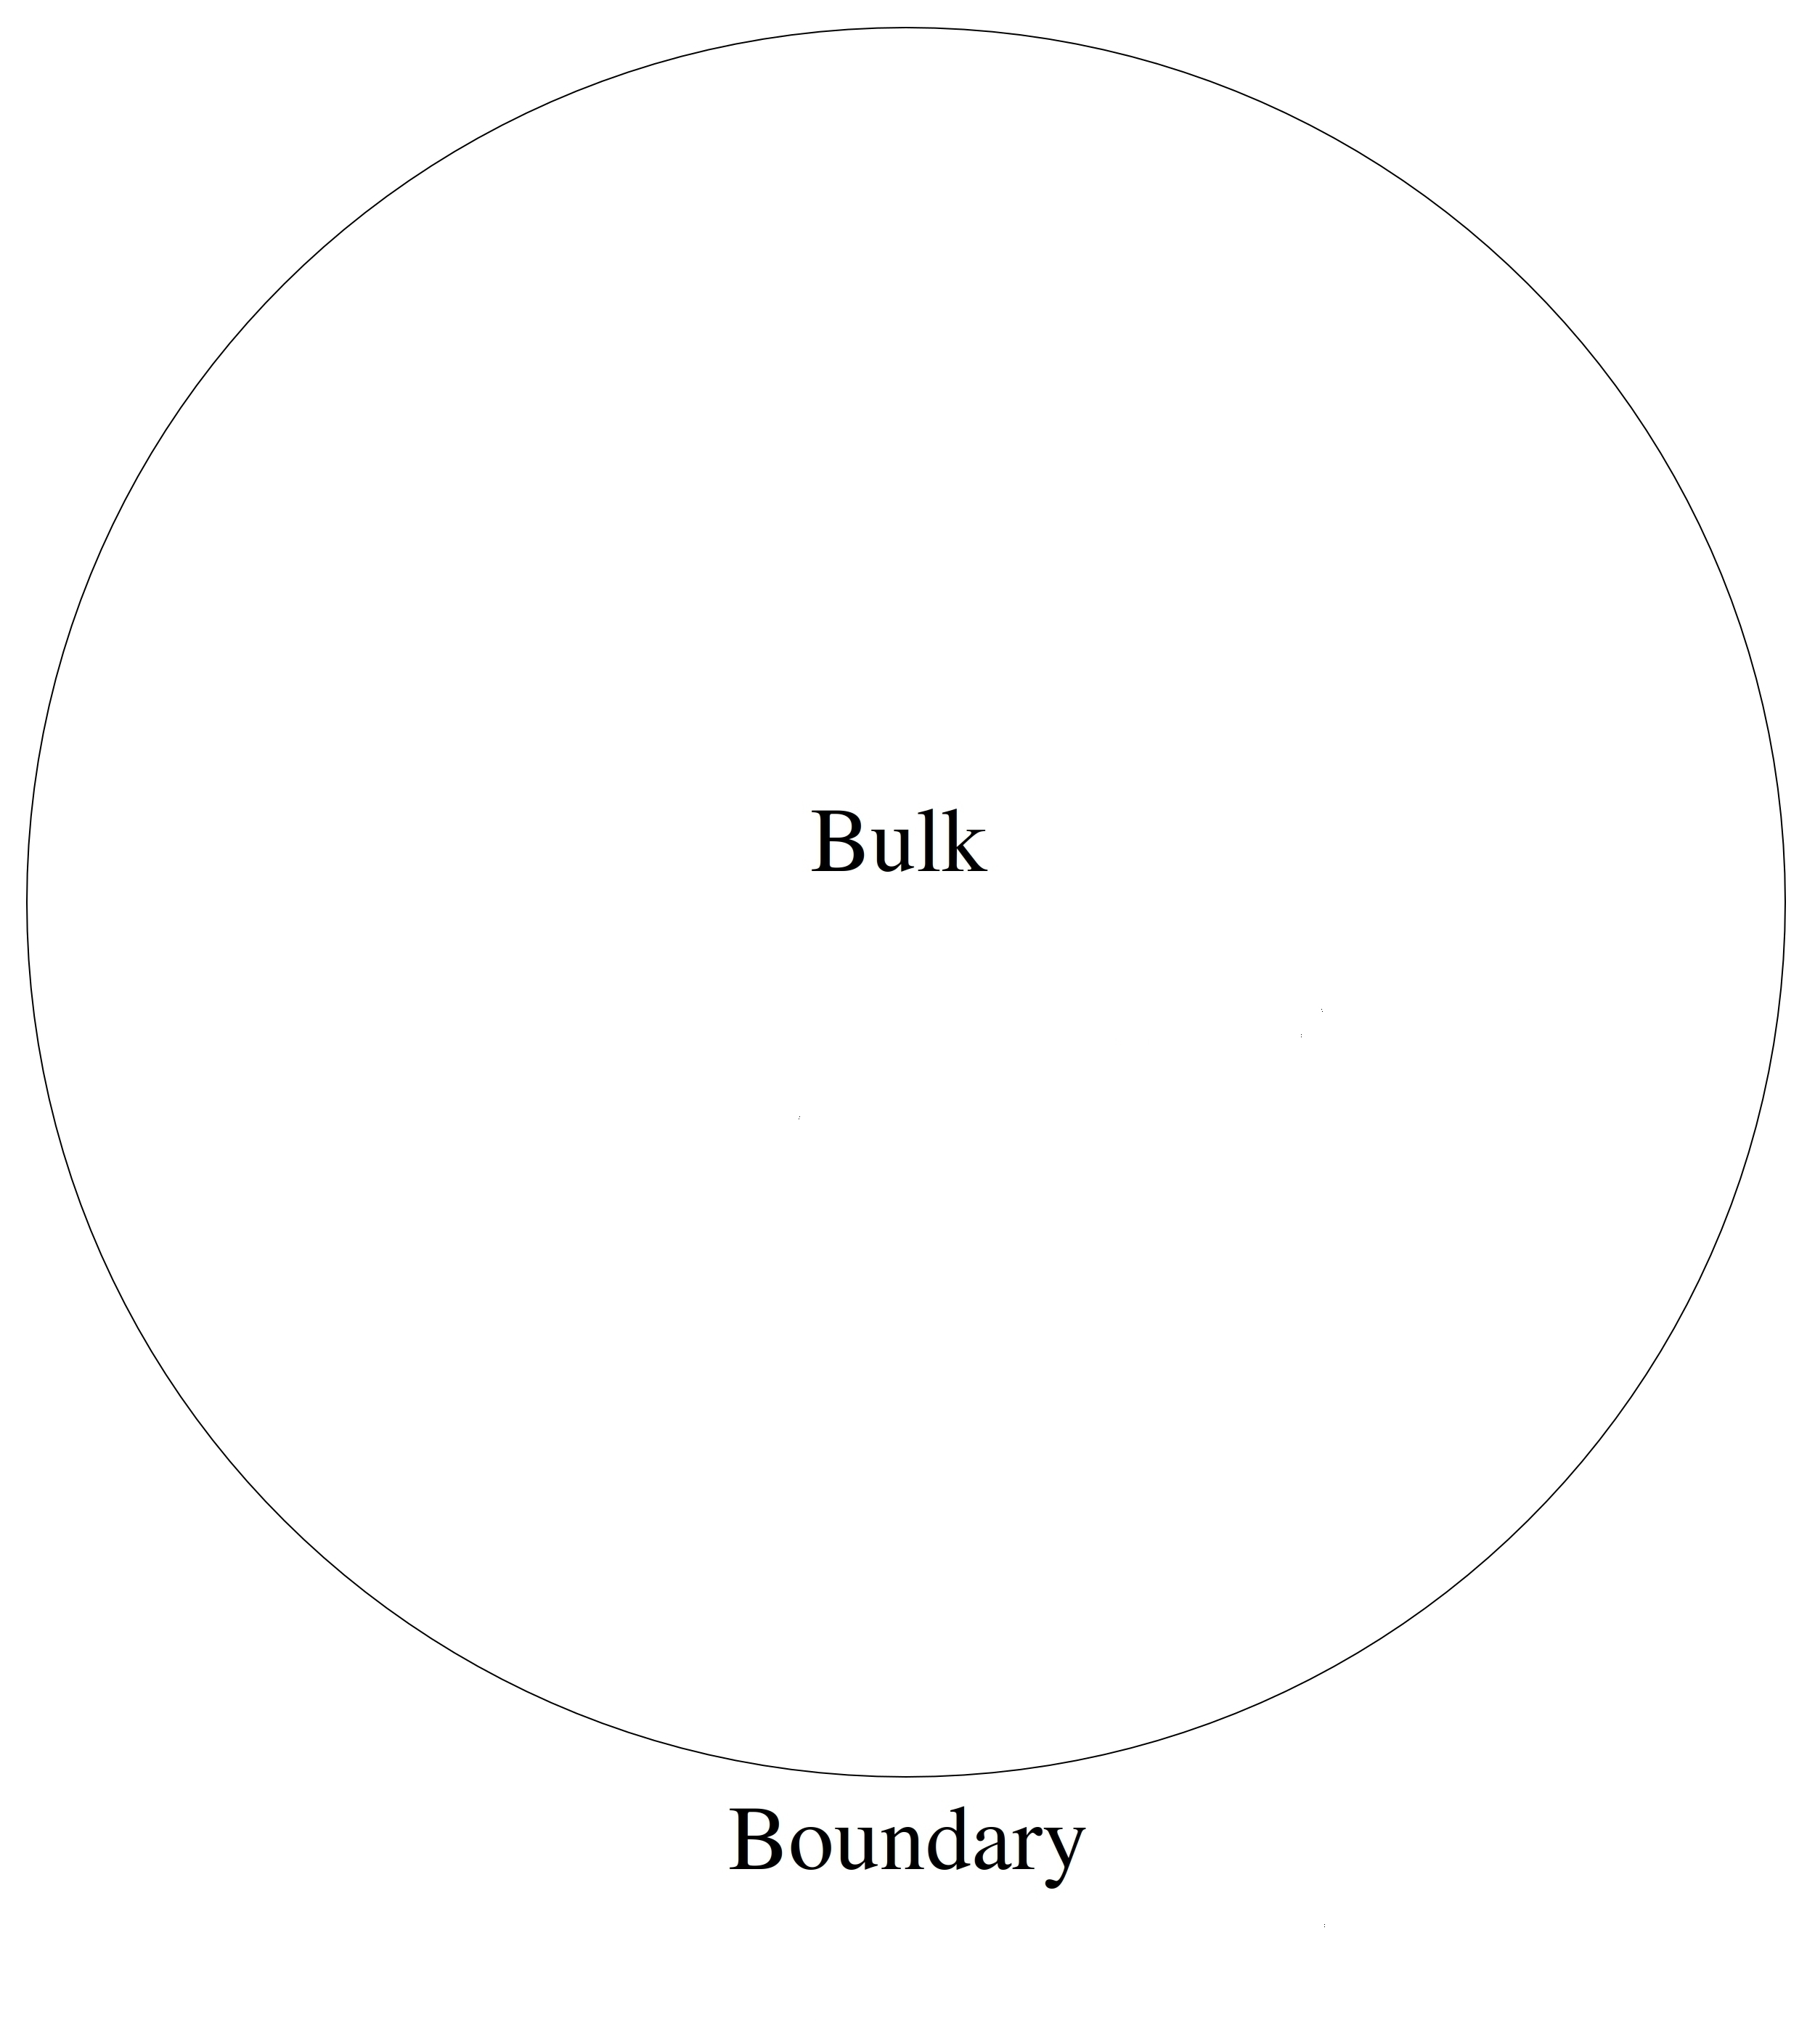
\includegraphics[scale=0.06]{adscft}    
    
    \end{center}
    \caption{The AdS/CFT Correspondence}
    \label{fig:WDW}
\end{figure}

\end{minipage}

\end{frame}

\begin{frame}
\frametitle{Holographic Complexity}

\begin{minipage}[t]{0.48\linewidth}

\begin{itemize}

\item Black holes are dual to thermal states.

\item Thermal state are in equilibrium, so observables don't generally evolve.

\item Yet, volume behind the horizon keeps growing. What could it be dual to?

\item Susskind suggested {\it quantum circuit complexity}

\item Complexity = Volume: the volume of a maximal spatial slice is dual to complexity.

\item Complexity = Action: The action on the Wheeler-DeWitt patch is dual to complexity

\item What evidence is there for this? Can we test it? 

\item Check field theory!

\end{itemize}

\end{minipage}
%
\hfill
%
\begin{minipage}[t]{0.48\linewidth}

\begin{figure}
    \begin{center}
    
        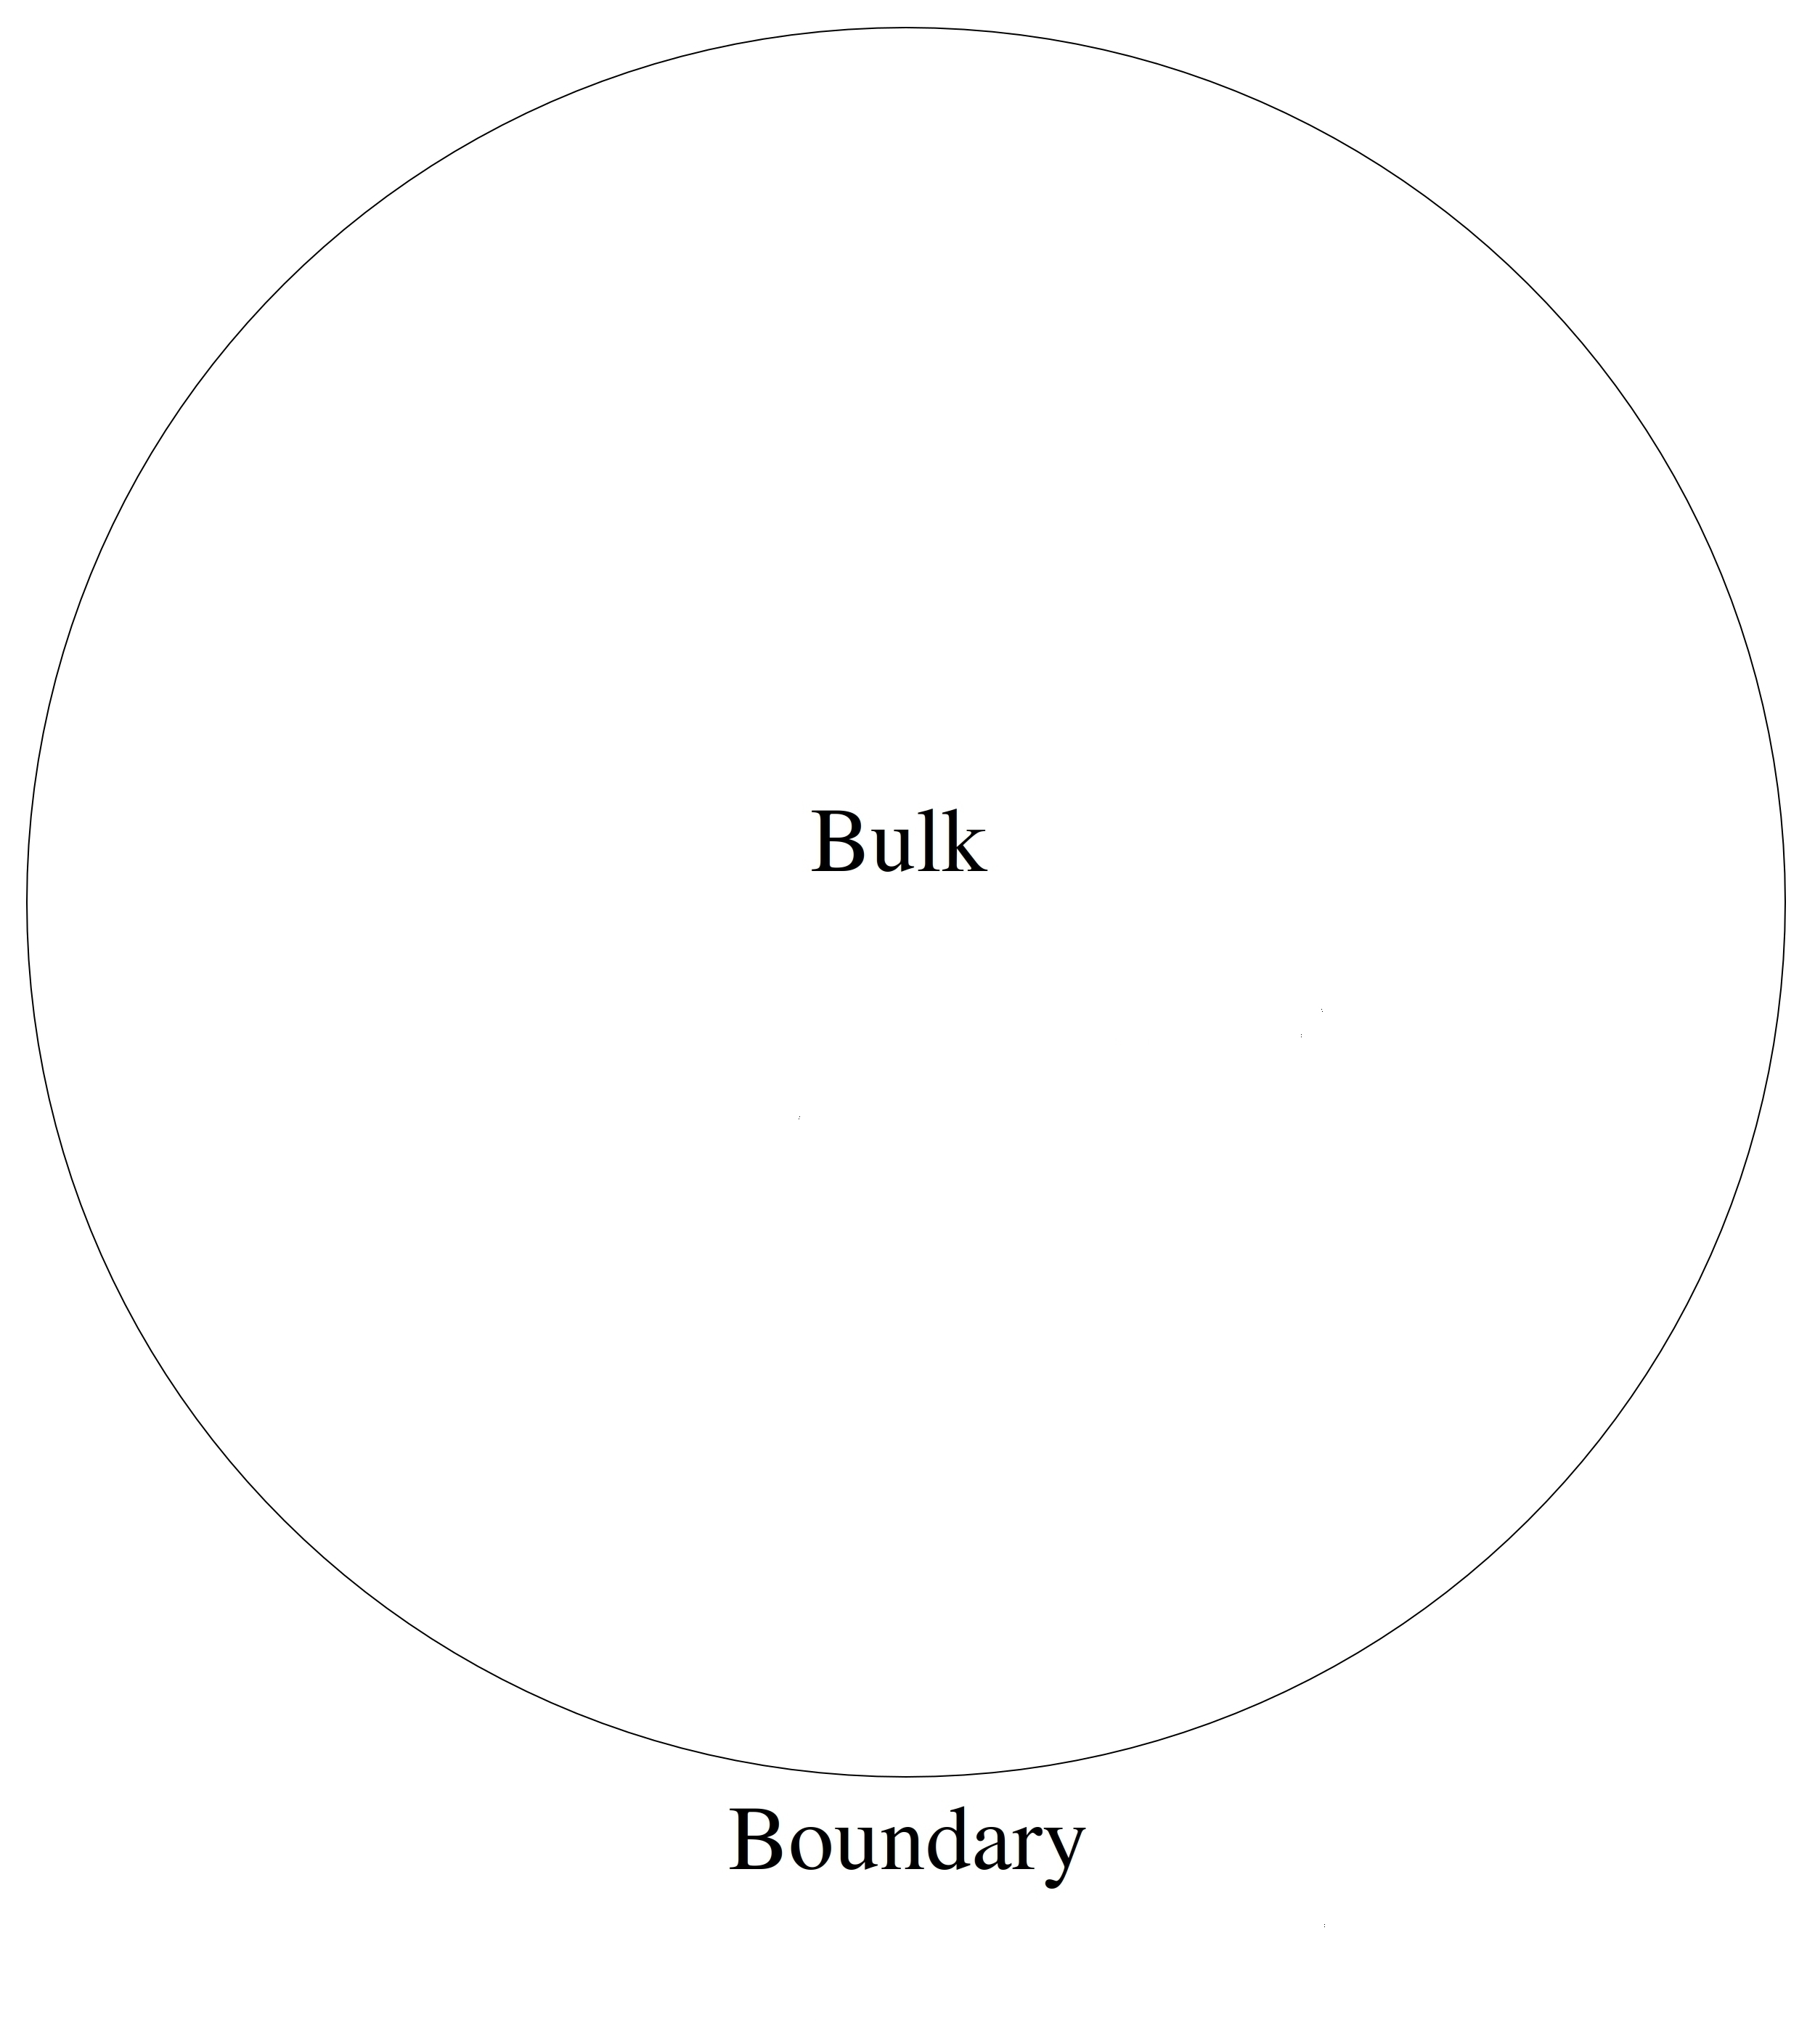
\includegraphics[scale=0.06]{adscft}    
    
    \end{center}
    \caption{The AdS/CFT Correspondence}
    \label{fig:WDW}
\end{figure}

\end{minipage}

\end{frame}

\begin{frame}
\frametitle{Circuit Complexity}

What is quantum circuit complexity?

\begin{itemize}

\item Consider a Hilbert space $\mathcal{H}$, e.g., the Hilbert space for $N$ quantum bits.

\item A universal gate set $\{g_i\}$ for $\mathcal{H}$ is a set of unitary operators on the Hilbert space such that any unitary $U$ acting on $\mathcal{H}$ can be approximated by some product $\displaystyle\prod_{i} g_{\alpha_i}$ to within a small tolerance $\epsilon$. 

\item Such a product of gates is referred to as a quantum circuit.

\item The quantum circuit complexity of a unitary $U$ is then the minimum number of gates needed to approximate $U$ to within the tolerance.

\item In the example of qubits, one typically considers gates that act on a single qubit or pairs of qubits at a time.

\item Given some reference state $\ket{\psi_R}$, one may define the complexity of a state $\ket{\psi}$ as the minimum of complexity $C(U)$ over all unitaries $U$ such that $\ket{\psi} = U\ket{\psi_R}$.

\end{itemize}

\end{frame}

\begin{frame}
\frametitle{Complexity in field theory?}

\begin{itemize}

\item Would like to compute the circuit complexity in the a CFT, and look for agreement.

\item Complexity in quantum field theories is not well understood, so just try to understand this.

\item Jefferson and Myers (2017) and Chapmap et al. (2017): Start with free scalar field theory in 1+1.

\item Actually, start with just lattice of harmonic oscillators.

\item consider Gaussian reference state, $\ket{R} \propto e^{-\frac{1}{2} \omega_0 |\vec{x}|^2}$, and gates which only take Gaussian states to other Guassian states. 

\item Reduce problem to finding geodesics by going to 'complexity geometry'

\item Jefferson and Myers found that for a state with normal modes $\omega_i$, 

$$ C = \sum_{i=1}^N \log\left| \frac{\omega_i}{\omega_0}\right|$$ 

\end{itemize}

\end{frame}

\begin{frame}
\frametitle{Subregion Complexity and Purification Complexity}

Subregion Complexity:

\begin{itemize}

\item Apply holographic complexity inside of the entanglement wedge (EW)

\item Since EW is dual to subregion, perhaps this 'subregion complexity' is dual to complexity of reduced state?

\item But what does complexity mean for a mixed state?

\item One definition (among many possible), suggested as promising by Ag\'on et al. (2018) is {\it purification complexity}

\end{itemize}

Purification Complexity:

\begin{itemize}

\item Given a mixed state $\rho$, and the set $\mathcal{P}$ of all purifications of $\rho$, the purification complexity of $\rho$ is 

$$C^P(\rho) = \text{min}_{\ket{\psi}\in \mathcal{P}} C(\ket{\psi})$$

\item Actually, we should restrict to only consider purifications $\ket{psi}$ such that all auxiliary systems are entangled with original system.

\end{itemize}

\end{frame}

\begin{frame}
\frametitle{Purification complexity in Field Theory}

Can we compute purification complexity in FT?

\begin{itemize}

\item Well, we can do small numbers of harmonic oscillators. Start with one.

\item Consider arbitrary Gaussian mixed state

$$\rho(x,x') := \bra{x} \rho \ket{x'} \propto e^{-\frac{1}{2}[a (x^2 + x'^2) - 2 b x x']}$$

\item An arbitrary purification to two oscillator state looks like

$$\psi(x) \propto e^{-\frac{1}{2} (\omega_1 x_1^2 + \omega_2 x_2^2 - 2\beta x_1 x_2)}$$

\item To be a purification of the mixed state above, we must require

$$\omega_1 = a - b \text{; } \beta = \sqrt{b \omega_2}$$

\item $\omega_2$ may be freely chosen, we will vary it to minimize the complexity of this purification.

\item Normal modes:

$$\omega_{\pm} = \frac{1}{2} \left[a-b + \omega_2 \pm \sqrt{\left( \omega_2 + b - a \right)^2  - 4 b \omega_2} \right]$$

\end{itemize}

\end{frame}

\begin{frame}
\frametitle{Purification Complexity in FT (continued)}

\begin{itemize}

\item We can now minimize $\log \left|\frac{\omega_+}{\omega_0} \right| + \log \left| \frac{\omega_-}{\omega_0} \right|$ over $\omega_2$.

\item But is this enough? Do we need to consider all purifications to 3 particle states? 4 particles?

\item Numerical studies seem to indicate that we get no smaller complexity from 3-particle purifications. Hopefully this result extrapolates to $N$ particles.

\item Can we do this for a whole lattice? 

\begin{itemize}

	\item Can write down arbitrary purification, find normal modes, and try minimization.
	
	\item But we are minimizing over a high dimensional space, so computationally hard
	
	\item Can 'cheat' by distilling entangled d.o.fs and purifying them pairwise.
	
	\item But in general, the cheat does not yield the global minimum. It is still an upper bound though.

\end{itemize} 

\item Ultimately, we aim to compute the complexity of a (regulated) field theory subregion, and compare the result to holographic subregion complexity.

\begin{itemize}
	
	\item Consider lattice of harmonic oscillators in ground state, and trace out all sites not in a given interval.
	
	\item Study dependence on cutoff (lattice spacing)
	
	\item Compare to subregion complexity of an interval of the boudary of $AdS_3$.	
	
	\item This is work in progress.
	
\end{itemize}

\end{itemize} 

\end{frame}

~~~~~~~~~~~~~~~~~~~~~~~~~~~~~~~~~~~~~~~~~~~~~~~~~~~~~~

\begin{frame}
\frametitle{Introduction}

Around 2014, Leonard Susskind and collaborators proposed a new entry in the {\color{blue} AdS/CFT dictionary}, namely that the volume of a maximal spatial slice of of asymptotically AdS spacetime is dual {\color{red} quantum circuit complexity} in the dual CFT.

%\hfill

\begin{minipage}[t]{0.48\linewidth}

{\color{blue} The AdS/CFT correspondence}:

\begin{itemize}

	\item Duallity between quantum gravity in $d+1$ dimensions and a conformal field theory in $d$ dimensions.
	
	\item The gravity theory lives on an Asymptotically $AdS$ (constant negative curvature) spacetime. 
	
	\item Relates weakly coupled gravity to strongly coupled CFT, and classical limit of gravity to limit of CFT with infinite d.o.fs.
	
	\item Quantities/observables from the CFT are related to those in the gravity theory and vice versa through the {\it 'dictionary'}.

\end{itemize}

\end{minipage}\hfill
%
\begin{minipage}[t]{0.48\linewidth}

{\color{red} Quantum Circuit Complexity}:

\begin{itemize}

	\item Consider a Hilbert space $\mathcal{H}$, e.g., the Hilbert space for $N$ quantum bits, and a (computationally) universal set of unitary {\it gates} $\{g_i\}$ on $\mathcal{H}$

	\item Consider also a reference state $\ket{R}$
	
	\item A product of gates $Q = \prod_i g_i$ is a quantum circuit, whose complexity is the number of gates in the product.
	
	\item Then the circuit complexity of a state $\ket{\psi}$ is the minimum complexity over all circuits $Q$ such that $\ket{\psi} = Q \ket{R}$

\end{itemize}

\end{minipage}

\end{frame}

\begin{frame}
\frametitle{Holographic Complexity}

So why would circuit complexity have anything to do with volume, anyway? Susskind was motivated by certain facts about the behind the horizon geometry of AdS black holes:

\begin{itemize}

\item (Large) black holes are dual to thermal states on the boundry. Two sided black holes are dual to a purification of the thermal state, the thermofield double state: $\ket{\text{TFD}} = \displaystyle\sum_n e^{- \beta E_n /2} \ket{n} \otimes \ket{n}$

\item The volume behind the black hole horizon increases in time, yet ordinary field theory obervables are not normally time dependent in a thermal state.

\item However, we expect the {\it circuit complexity} of the TFD state to increase under time evolution, like the volume

\item The volume also also reproduces the so-called {\it switchback effect}, an effect complexity is expected to exhibit.

\item With a proper choice of normalization constant, the 'holographic complexity' computed by volume grows like $T S$ at late time. This matches the behavior expected of complexity based on circuit arguments. 

\end{itemize}

Susskind later updated his conjecture to 'complexity = action', in which complexity is instead thought to be dual to the causal development of such a maximal slice, termed the Wheeler-DeWitt (WDW) patch.

\end{frame}

\begin{frame}
\frametitle{Complexity in field theory?}

While we have some indication holographic complexity {\it might} be correct, stronger evidence is needed before it is accepted as a valid entry in the AdS/CFT dictionary.

\begin{itemize}

\item Ideally we would compute the circuit complexity in the a CFT, and look for agreement.

\item However, complexity in quantum field theories (as opposed to systems of qubits) is not well understood, so as a first step, we should understand circuit complexity in field theories.

\item In the past two years or so, there has been progress towards this, by e.g. Hashimoto et al. (2017) in for lattice gauge theory, and by Jefferson et al. (2017) and Chapmap et al. (2017) respectivley for lattice regularized scalar FT.

\item In particular, Jefferson et al. considered Guassian states of harmonic oscillators, and a gate set which, though not universal, is at least universal on Gaussian states, and a reference state

$$\ket{R} \propto e^{-\frac{1}{2} \omega_0 |\vec{x}|^2}$$ 

\item They found that the complexity of a Gaussian state on $N$ oscillators, with normal mode frequencies $\omega_i$, is given by 

$$ C = \sum_{i=1}^N \log\left| \frac{\omega_i}{\omega_0}\right|$$ 

\end{itemize}

\end{frame}

\begin{frame}
\frametitle{Subregion Complexity and Purification Complexity}

Subregion Complexity:

\begin{itemize}

\item It is widely believed that the reduced state on a subregion of the CFT is dual to the bulk {\it entanglement wedge} associated to that region. This is called subregion duality.

\item We may apply the holographic complexity conjectures to the entanglement wedge just as easily as to the whole geometry.

\item The resulting quantity is termed {\it subregion complexity}. It is conjectured that it is dual to some notion of complexity on the reduced state.

\item However, there is not a unique way to extend the definition of complexity to mixed states.

\end{itemize}

Purification Complexity:

\begin{itemize}

\item Recently, Ag\'on et al. studied different definitions of mixed state complexity, and compared expectations about them to holographic subregion complexity.

\item They suggested that the closest match to holographic complexity (in its complexity = action form, anyway) was the {\it purification complexity}.

\item The purification complexity of a state $\rho$ is defined as the minimum complexity $C(\ket{\psi})$ over all purifcations $\ket{\psi}$ of $\rho$, which don't have any seperable factor which is also a purification of $\rho$.

\end{itemize}

\end{frame}

\begin{frame}
\frametitle{Purification complexity in field theory}

Can we compute purification complexity in FT?

\begin{itemize}

\item Well, we can do small numbers of harmonic oscillators.

\item Hard to minimize over all purifcations $\rightarrow$ try just those of on to copies of original Hilbert space. Is this enough?

\item Parameterize all purifications to the Guassian state, and numerically minimize the complexity as found by Jefferson et al.

$$C = \sum_i \log \left| \frac{\omega_i}{\omega_0} \right|$$

\item Consider mixed states that come by tracing out all but a few sites on a lattice, as well as thermal states

\item Compare result to holographic computation.

\end{itemize}

\end{frame}

\begin{frame}
\frametitle{Results}

\begin{itemize}

\item It seems one doesn't need extra factors of the Hilbert space, e.g. purifying one oscillator onto three doesn't seem to improve on purifying to two (No proof though).

\end{itemize}

\end{frame}

\end{document}